\documentclass[xcolor={table}]{beamer}
\usetheme{Singapore}
\usepackage[utf8]{inputenc}
\usecolortheme{crane}
\usepackage{graphicx}
\usepackage{iwona}
\usepackage{standalone}
\usepackage{tikz}
\usetikzlibrary{arrows}
\usetikzlibrary{decorations.markings}
\usetikzlibrary{calc}
\usetikzlibrary{shapes,snakes}
\usepackage{amsmath}
\usepackage{amsfonts}
\usepackage{amsthm}
\usepackage{mathtools}

\definecolor{lightblue}{RGB}{124,190,255}
\definecolor{darkgreen}{RGB}{24,145,0}

\beamertemplatenavigationsymbolsempty
\setbeamerfont{caption}{size=\tiny}


\title{Deadlock in Open Restricted Queueing Networks}
\author{Geraint Palmer\newline \scriptsize{Prof. Paul Harper \& Dr. Vincent Knight}}
\date{13\textsuperscript{th} March 2017}
\titlegraphic{
\includegraphics[width=2cm]{../cflogo.pdf}}

\begin{document}
\frame{\titlepage}

\begin{frame}
  \frametitle{Deadlock}
    \begin{figure}
    \includestandalone[width=0.7\textwidth]{../images/gridlock}
    \end{figure}
\end{frame}

\begin{frame}
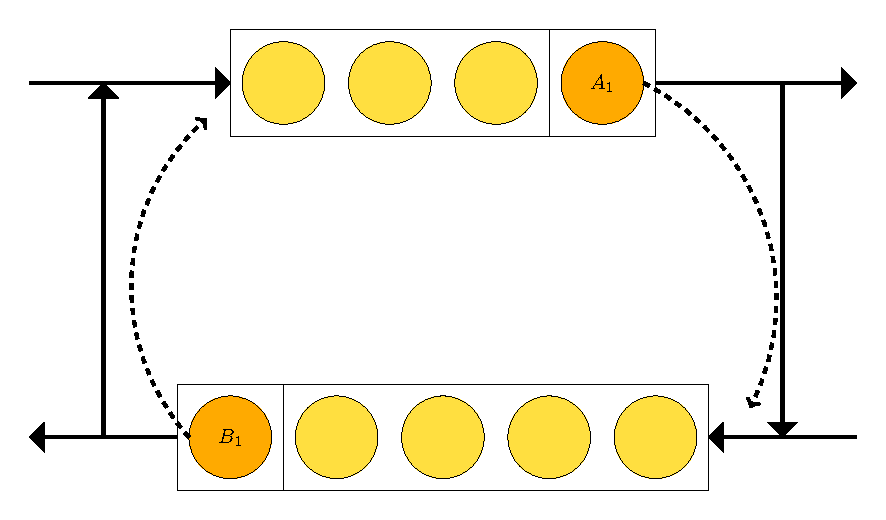
\includegraphics[width=\textwidth]{../images/2nodesindeadlock.pdf}
\end{frame}


\begin{frame}
    \begin{figure}
    \includestandalone[width=\textwidth]{../images/buildupdigraph}
    \end{figure}
\end{frame}

\begin{frame}
    \frametitle{Markovian Model of Deadlock}
    \includestandalone[width=\textwidth]{../images/1nodemultiserver}\newline
    \center{\LARGE{$(i)$}}
\end{frame}

\begin{frame}
\center
\scriptsize  \[S = \{i\in\mathbb{N} \nonscript\; | \nonscript\; 0 \leq i \leq n + 2c\}\]
Define $\delta = i_2 - i_1$\newline

\vspace{10 mm}

  $  q_{i_1, i_2} = \left\{
  \begin{matrix*}[ r ]
    \left. \begin{matrix*}[ r ]
      \color{red} \Lambda & \color{red} \text{if } \delta = 1 \\
      \color{blue} (1-r_{11})\mu\text{min}(i, c) & \color{blue} \text{if } \delta = -1 \\
      0 & \text{otherwise}
    \end{matrix*} \right\} & \text{if } i_1 < n + c \\
  \end{matrix*} \right.
$
\vspace{10 mm}

  $q_{i_1, i_2} = \left\{
  \begin{matrix*}[ r ]
    \left. \begin{matrix*}[ r ]
      \color{darkgreen} (c-b)r_{11}\mu & \color{darkgreen} \text{if } \delta = 1 \\
      \color{blue} (1-r_{11})(c-b)\mu & \color{blue} \text{if } \delta = -b-1\\
      0 & \text{otherwise}
    \end{matrix*} \right\} & \text{if } i_1 = n + c + b \\
  \end{matrix*} \right.
  \quad \forall \quad 0 \leq b \leq c$

\vspace{10 mm}
\end{frame}

\begin{frame}
    \begin{figure}
    \includestandalone[width=0.95\textwidth]{../images/MC1nodemultiserv}
    \end{figure}
\end{frame}

\begin{frame}
    \frametitle{Times to Deadlock}
    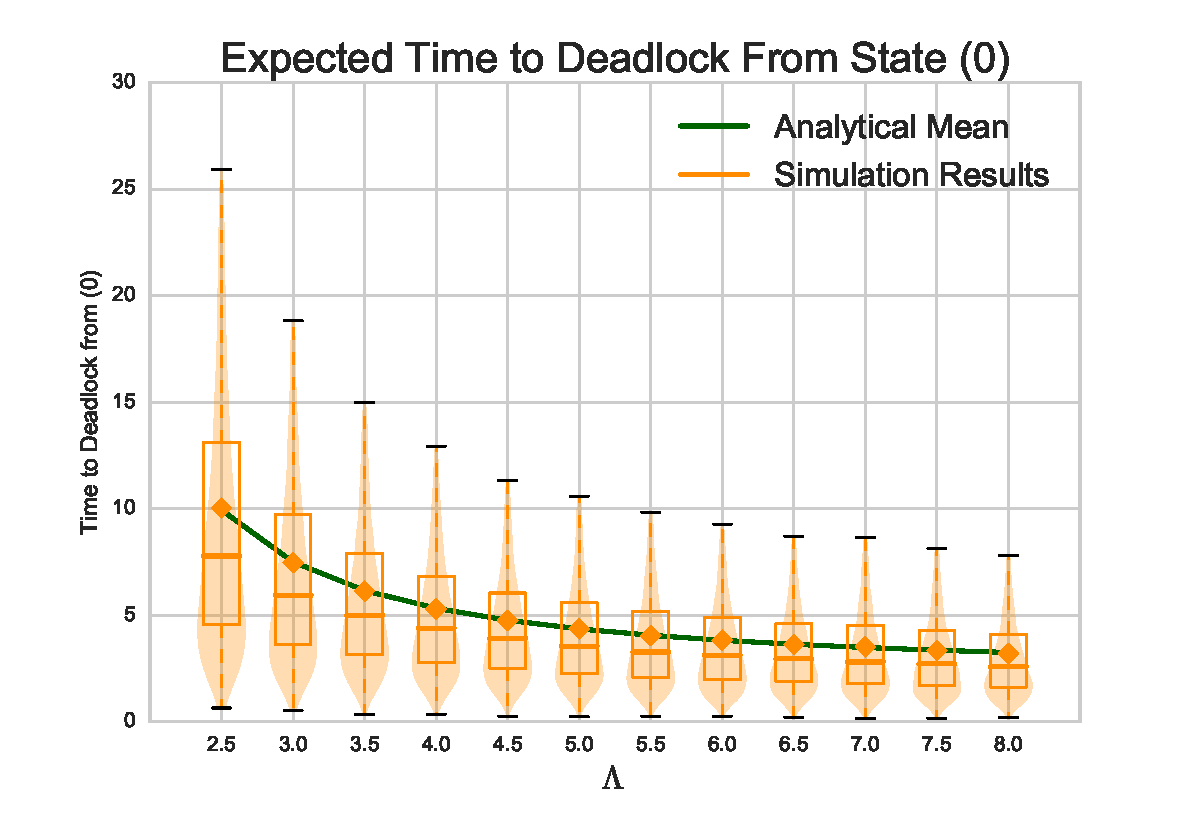
\includegraphics[width=0.5\textwidth]{../images/varyL_1Nms}
    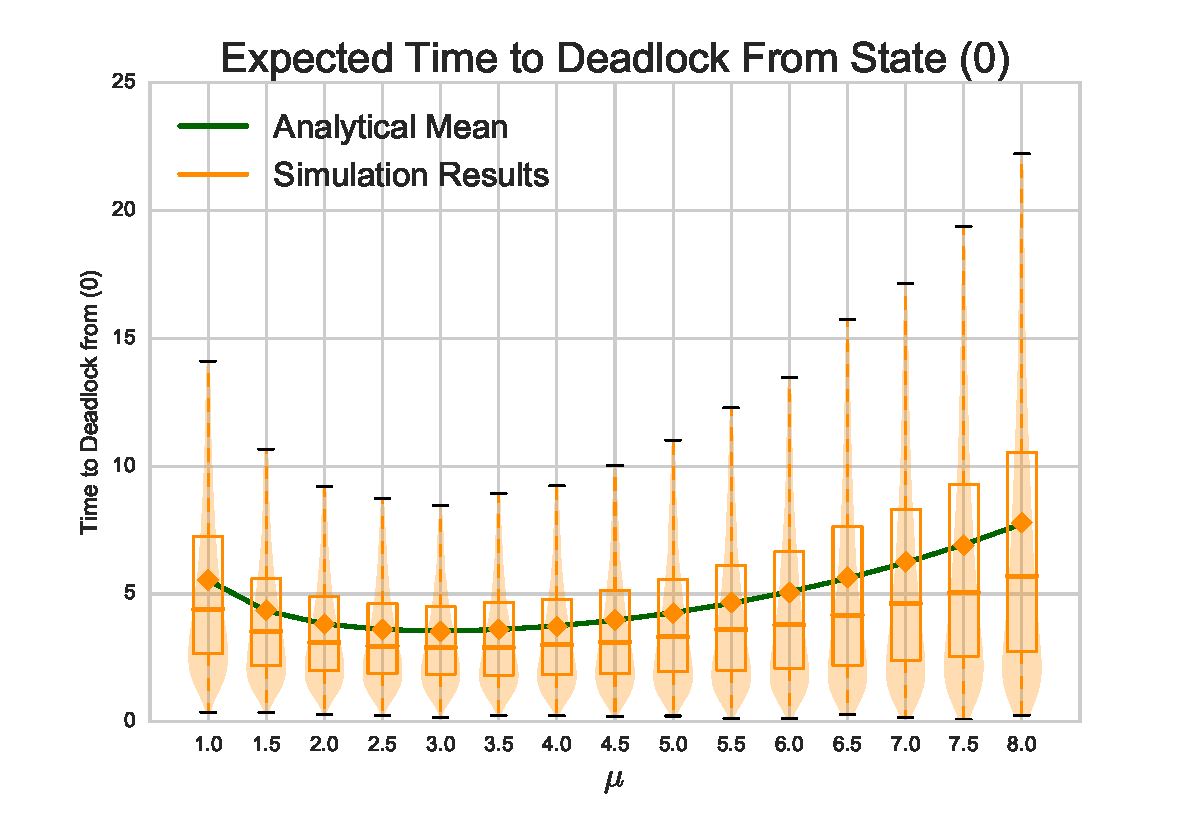
\includegraphics[width=0.5\textwidth]{../images/varymu_1Nms}\newline
    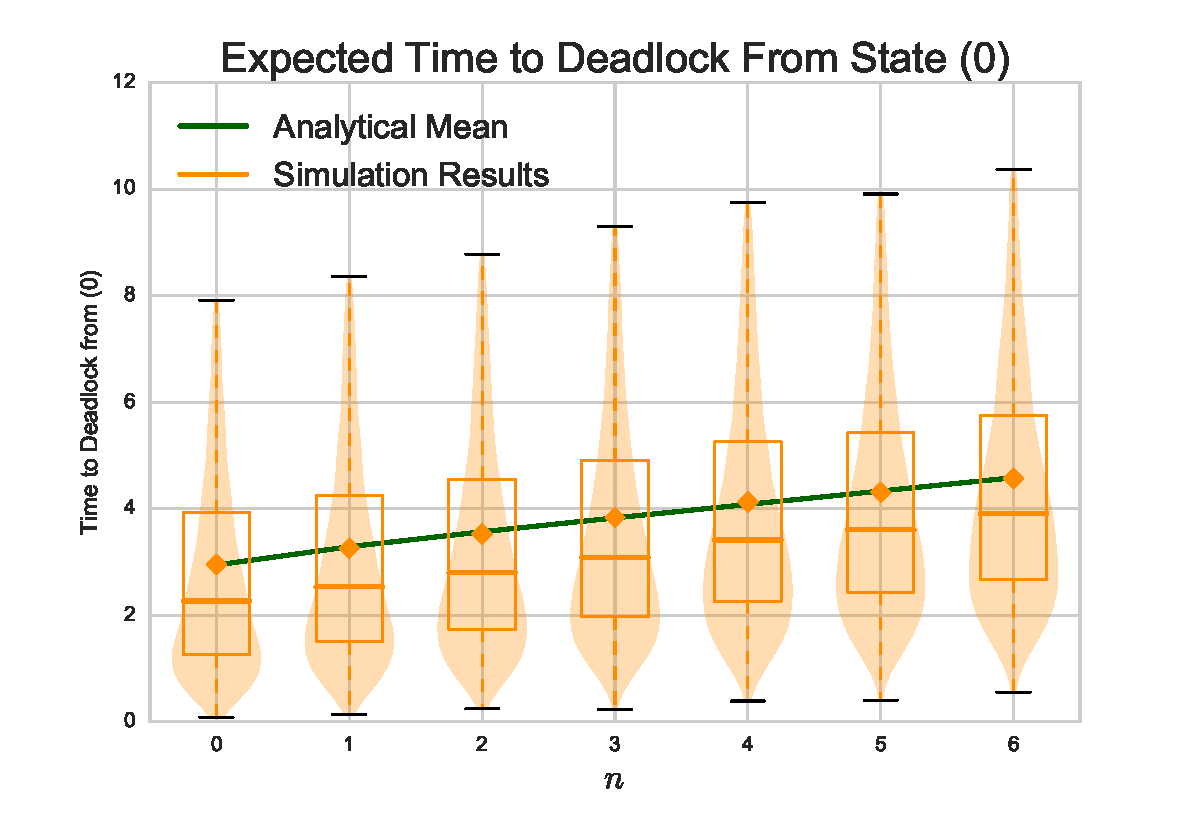
\includegraphics[width=0.5\textwidth]{../images/varyn_1Nms}
    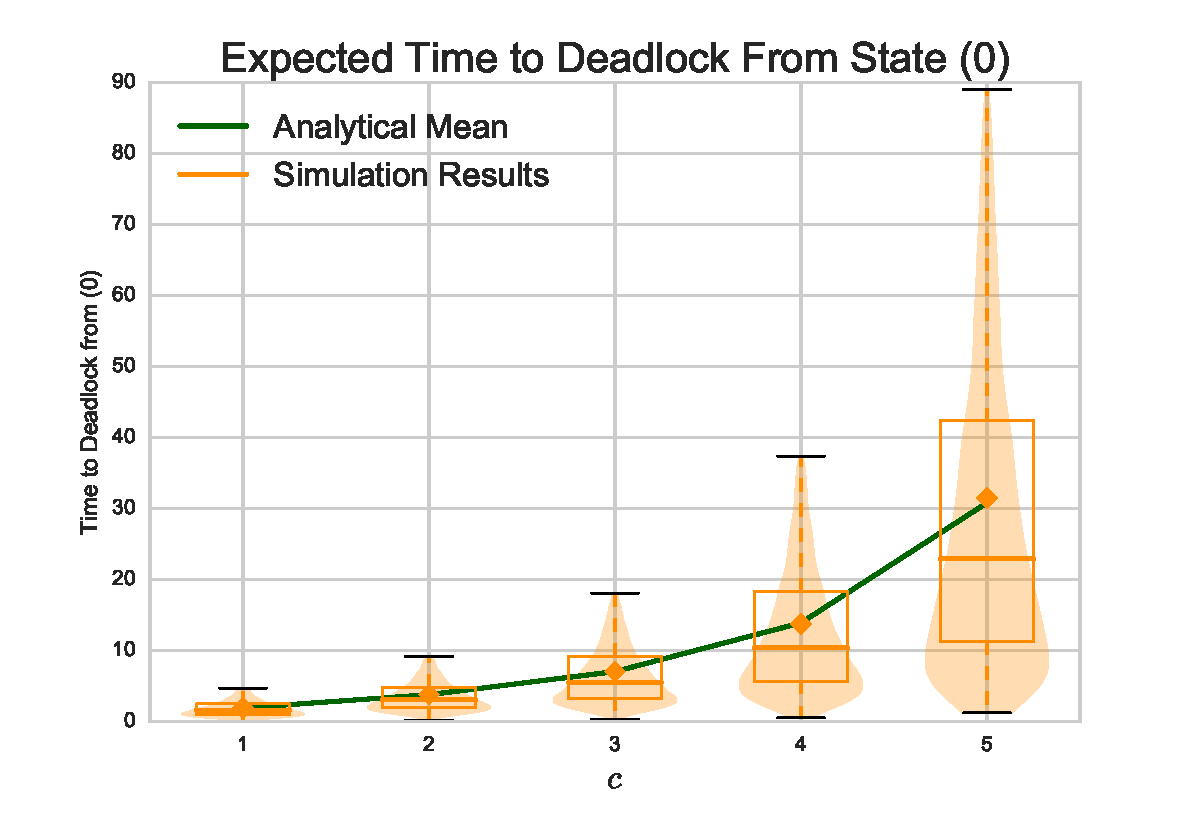
\includegraphics[width=0.5\textwidth]{../images/varyc_1Nms}
\end{frame}

\begin{frame}
    \frametitle{Markovian Model of Deadlock}
    \includestandalone[width=\textwidth]{../images/2nodefeedbackexample}\newline
    \center{\LARGE{$(i, j)$}}
\end{frame}


\begin{frame}
\center
\scriptsize \[S = \{(i,j)\in\mathbb{N}^{(n_1+2\times n_2+2)} \nonscript\; | \nonscript\; 0 \leq i + j \leq n_1 + n_2 + 2\}\cup\{(-1), (-2), (-3)\}\]
Define $\delta = (i_2, j_2) - (i_1, j_1)$\newline\newline
\tiny{
  $q_{(i_1, j_1),(i_2, j_2)} = \left\{
  \begin{matrix*}[ r ]
    \left. \color{red} \begin{matrix*}[ r ]
      \Lambda_1 & \text{if } i_1 \leq n_1 \\
      0 & \text{otherwise}
    \end{matrix*} \right\} & \color{red} \text{if } \delta = (1, 0)\\
    \left. \color{orange} \begin{matrix*}[ r ]
      \Lambda_2 & \text{if } j_1 \leq n_2 \\
      0 & \text{otherwise}
    \end{matrix*} \right\} & \color{orange} \text{if } \delta = (0, 1) \\
    \left. \color{blue} \begin{matrix*}[ r ]
      (1 - r_{12})\mu_1 & \color{blue} \text{if } j_1 < n_2 + 2 \\
      0 & \text{otherwise}
    \end{matrix*} \right\} & \color{blue} \text{if } \delta = (-1, 0) \\
    \left. \color{lightblue} \begin{matrix*}[ r ]
      (1 - r_{21})\mu_2 & \text{if } i_1 < n_1 + 2 \\
      0 & \color{lightblue} \text{otherwise}
    \end{matrix*} \right\} & \color{lightblue} \text{if } \delta = (0, -1) \\
    \left. \color{darkgreen} \begin{matrix*}[ r ]
      r_{12}\mu_1 & \text{if } j_1 < n_2 + 2 \text{ and } (i_1, j_1) \neq (n_1+2, n_2) \\
      0 & \text{otherwise}
    \end{matrix*} \right\} & \color{darkgreen} \text{if } \delta = (-1, 1) \\
    \left. \color{green} \begin{matrix*}[ r ]
      r_{21}\mu_2 & \text{if } i_1 < n_1 + 2 \text{ and } (i_1, j_1) \neq (n_1, n_2+2)\\
      0 & \text{otherwise}
    \end{matrix*} \right\} & \color{green} \text{if } \delta = (1, -1) \\
    0 & \text{otherwise}
  \end{matrix*} \right.$\newline\newline

  $q_{(i_1, j_1), (-1)} = \left\{
  \begin{matrix*}[ r ]
    \color{magenta!50} r_{11}\mu_1 & \color{magenta!50} \text{if } i > n_1 \text{ and } j < n_2 + 2 \\
    0 & \text{otherwise}
  \end{matrix*}
  \right.$\newline

  $q_{(i_1, j_1), (-2)} = \left\{
  \begin{matrix*}[ r ]
    \color{violet!50} r_{22}\mu_2 & \color{violet!50} \text{if } j > n_2 \text{ and } i < n_1 + 2 \\
    0 & \text{otherwise}
  \end{matrix*}
  \right.$\newline

  $q_{(i_1, j_1), (-3)} = \left\{
  \begin{matrix*}[ r ]
    \color{green} r_{21}\mu_2 & \color{green} \text{if } (i, j) = (n_1, n_2 + 2) \\
    \color{darkgreen} r_{12}\mu_1 & \color{darkgreen} \text{if } (i, j) = (n_1 + 2, n_2) \\
    0 & \text{otherwise}
  \end{matrix*}
  \right.$\newline

$q_{-1, s} = q_{-2, s} = q_{-3, s} = 0$
}
\end{frame}


\begin{frame}
    \begin{figure}
    \includestandalone[width=0.95\textwidth]{../images/markov_chain_feedback}
    \end{figure}
\end{frame}

\begin{frame}
    \frametitle{Times to Deadlock}
    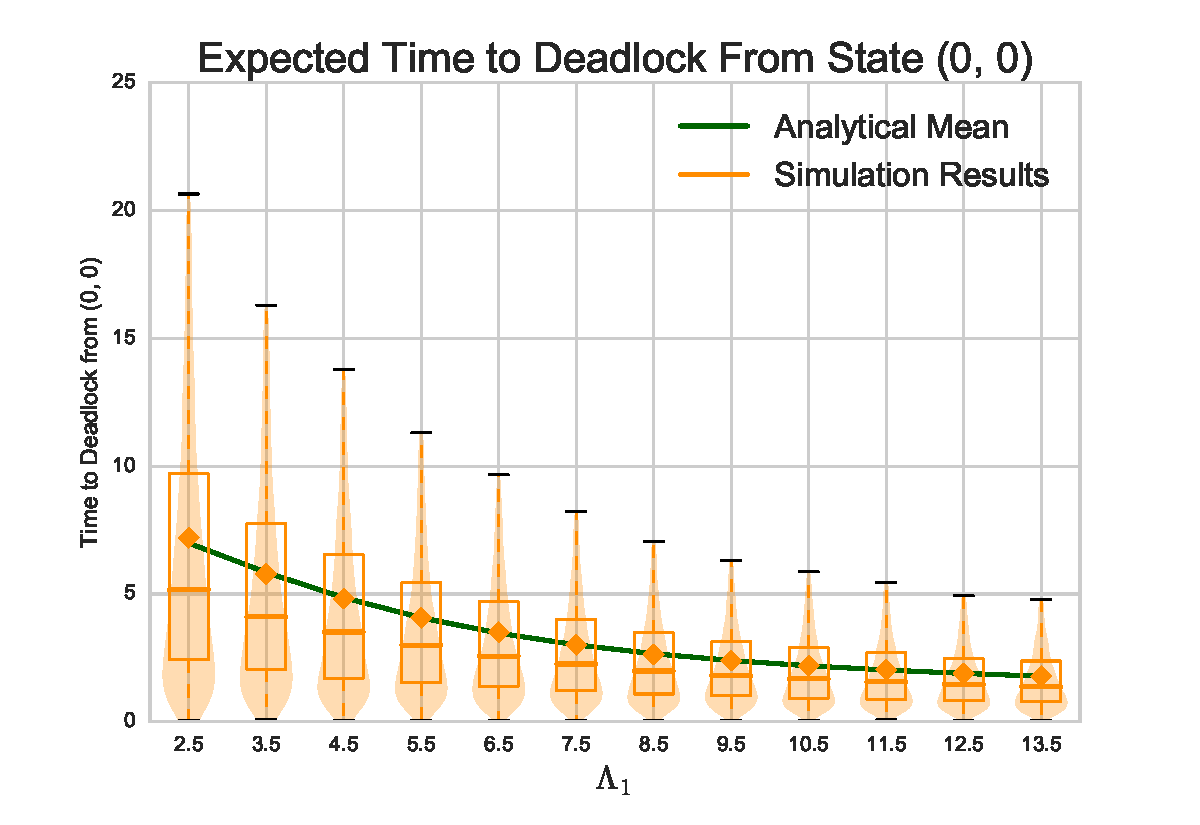
\includegraphics[width=0.5\textwidth]{../images/vary_L1fb}
    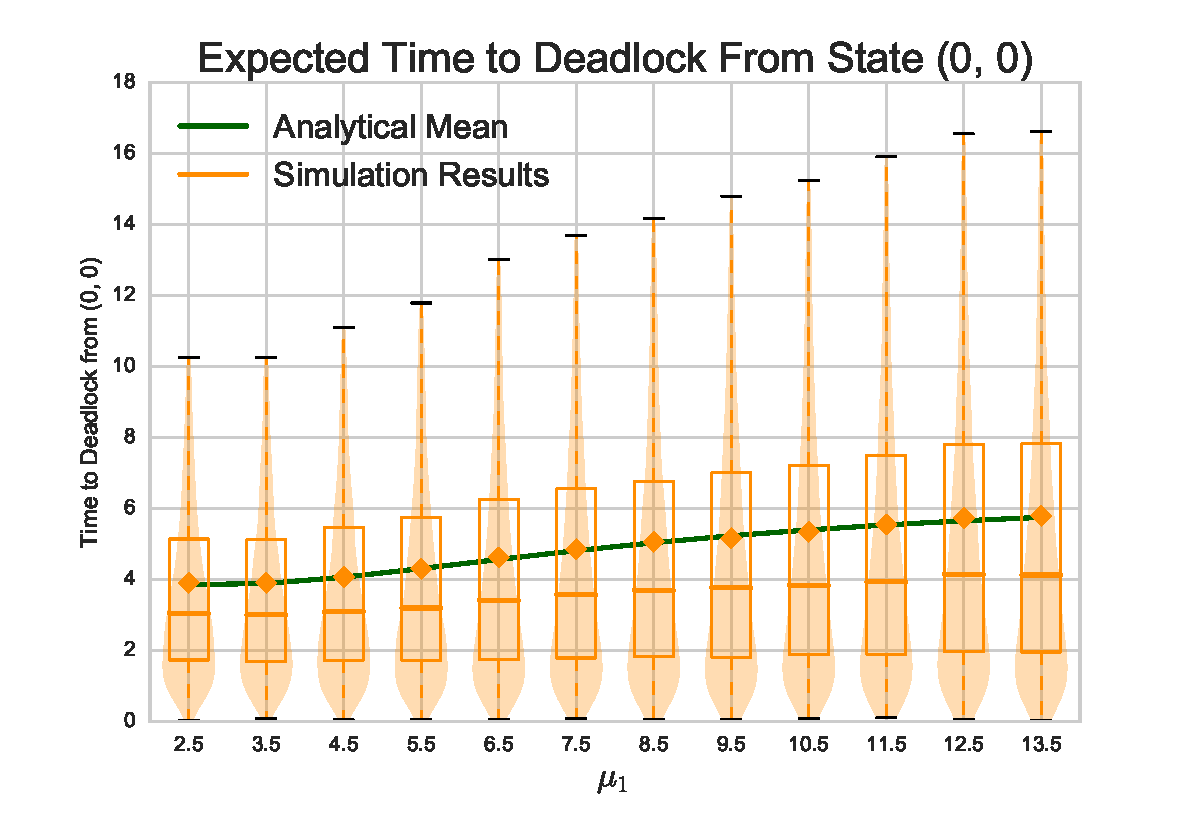
\includegraphics[width=0.5\textwidth]{../images/vary_mu1fb}\newline
    \centering
    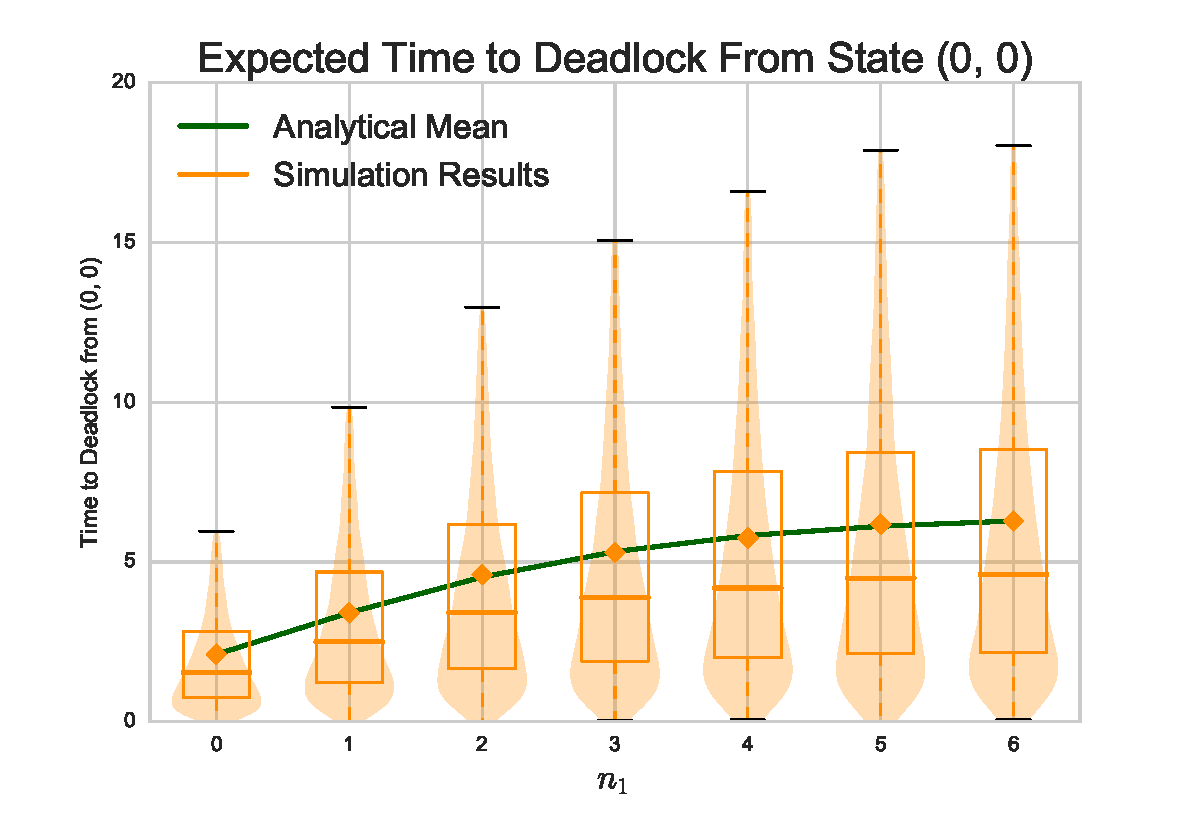
\includegraphics[width=0.5\textwidth]{../images/vary_n1fb}
\end{frame}

\begin{frame}
\begin{center}
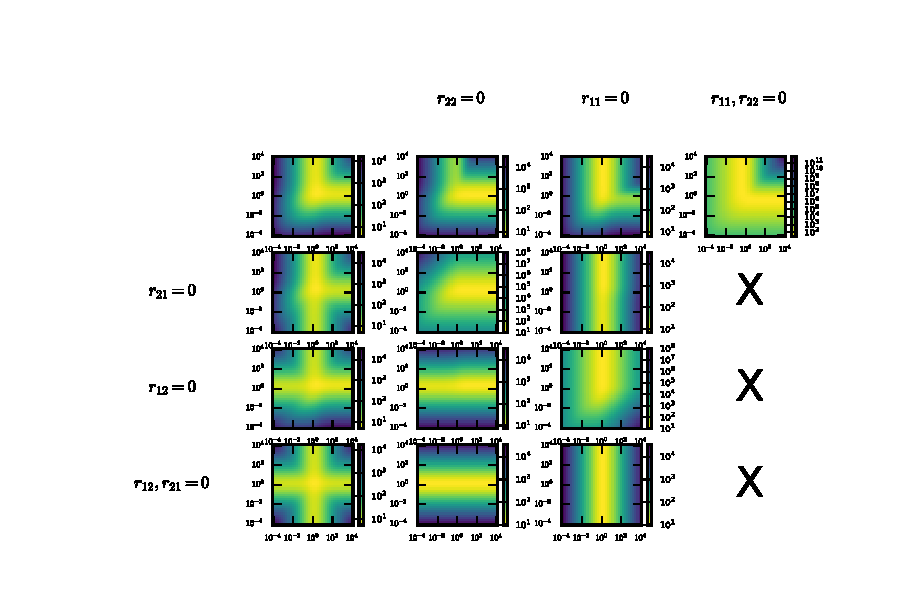
\includegraphics[width=0.95\textwidth]{../images/muslimit_allcombinations.pdf}
\end{center}
\end{frame}

\begin{frame}
  \frametitle{$\omega \leq \min(\omega_{1_1}, \omega_{1_2}, \omega_2)$}
  \begin{center}
  \includestandalone[width=0.45\textwidth]{../images/omega11}
  \includestandalone[width=0.45\textwidth]{../images/omega12}
  \includestandalone[width=0.45\textwidth]{../images/omega2}
  \end{center}
\end{frame}

\begin{frame}
\frametitle{Baulking}
\begin{equation*}
b_2(m) = \left\{ \begin{array}{rr}
0 & \text{if } m = 0\\
1 - \frac{\beta}{m} & \text{otherwise}
\end{array} \right.
\end{equation*}
\begin{center}
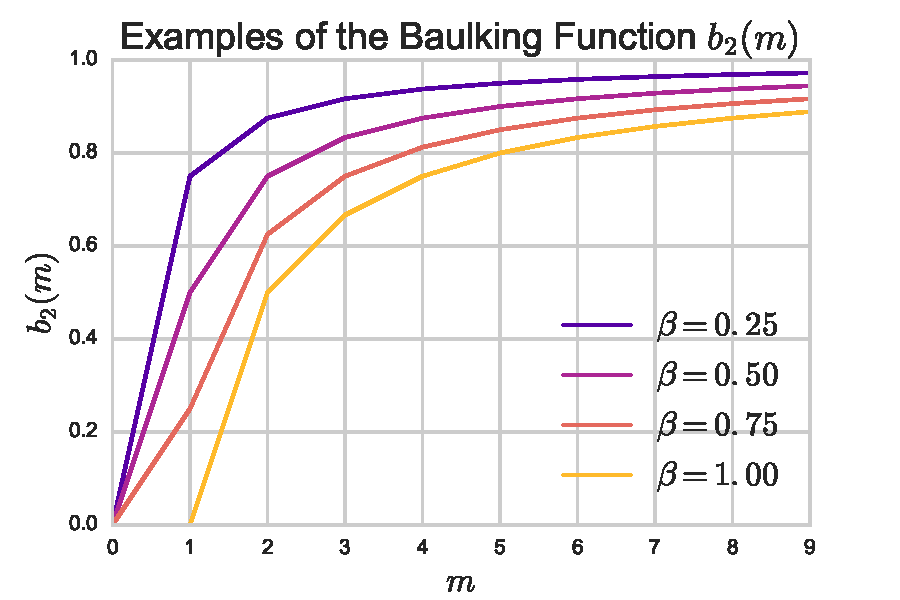
\includegraphics[width=0.75\textwidth]{../images/examplebaulking2.pdf}
\end{center}
\end{frame}

\begin{frame}
\frametitle{Baulking}
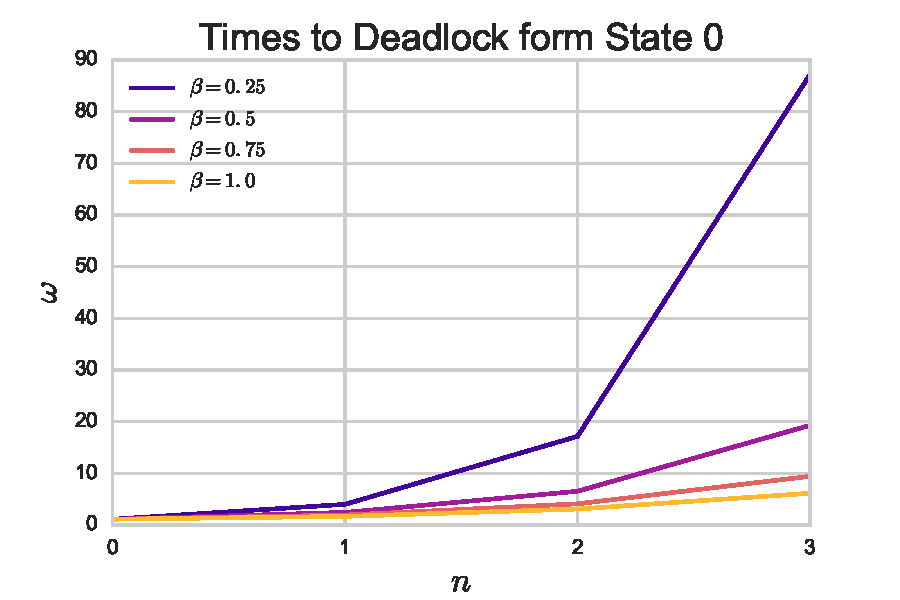
\includegraphics[width=0.5\textwidth]{../images/varyn_bybeta.pdf}
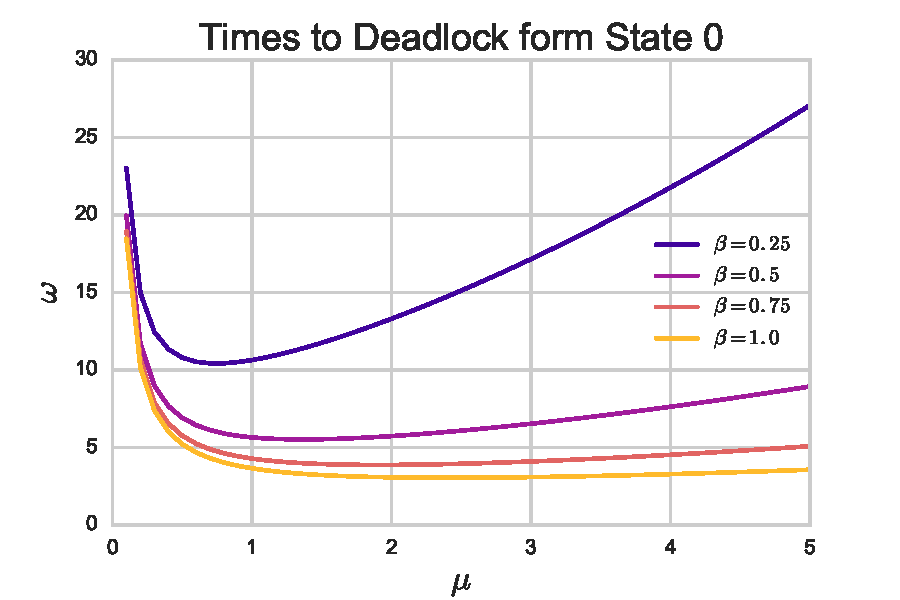
\includegraphics[width=0.5\textwidth]{../images/varymu_bybeta.pdf}
\end{frame}

\begin{frame}
\frametitle{Scheduled Vacations}
\includestandalone[width=\textwidth]{../images/onoffdutycycle}
\end{frame}

\begin{frame}
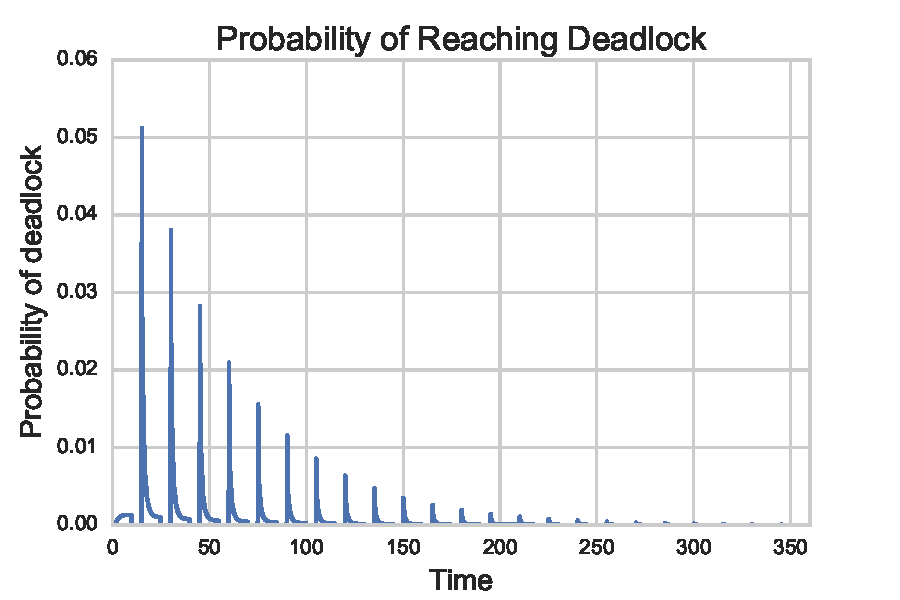
\includegraphics[width=0.5\textwidth]{../images/pdf_initial.pdf}
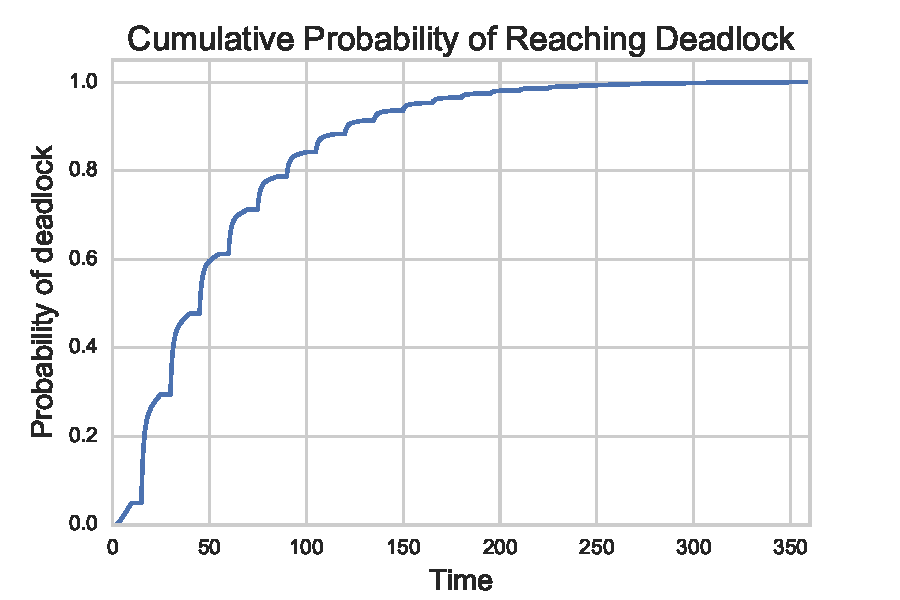
\includegraphics[width=0.5\textwidth]{../images/cdf_initial.pdf}
\end{frame}

\begin{frame}
\begin{center}
\includestandalone[width=0.95\textwidth]{../images/resolution_counterexample}
\end{center}
\end{frame}

\begin{frame}
\begin{center}
\includestandalone[width=0.8\textwidth]{../images/proceduremap}
\end{center}
\end{frame}

\begin{frame}
\begin{center}

\includegraphics[width=0.7\textwidth]{../images/example1_mdp.pdf}
\end{center}
\end{frame}

\begin{frame}
\begin{center}
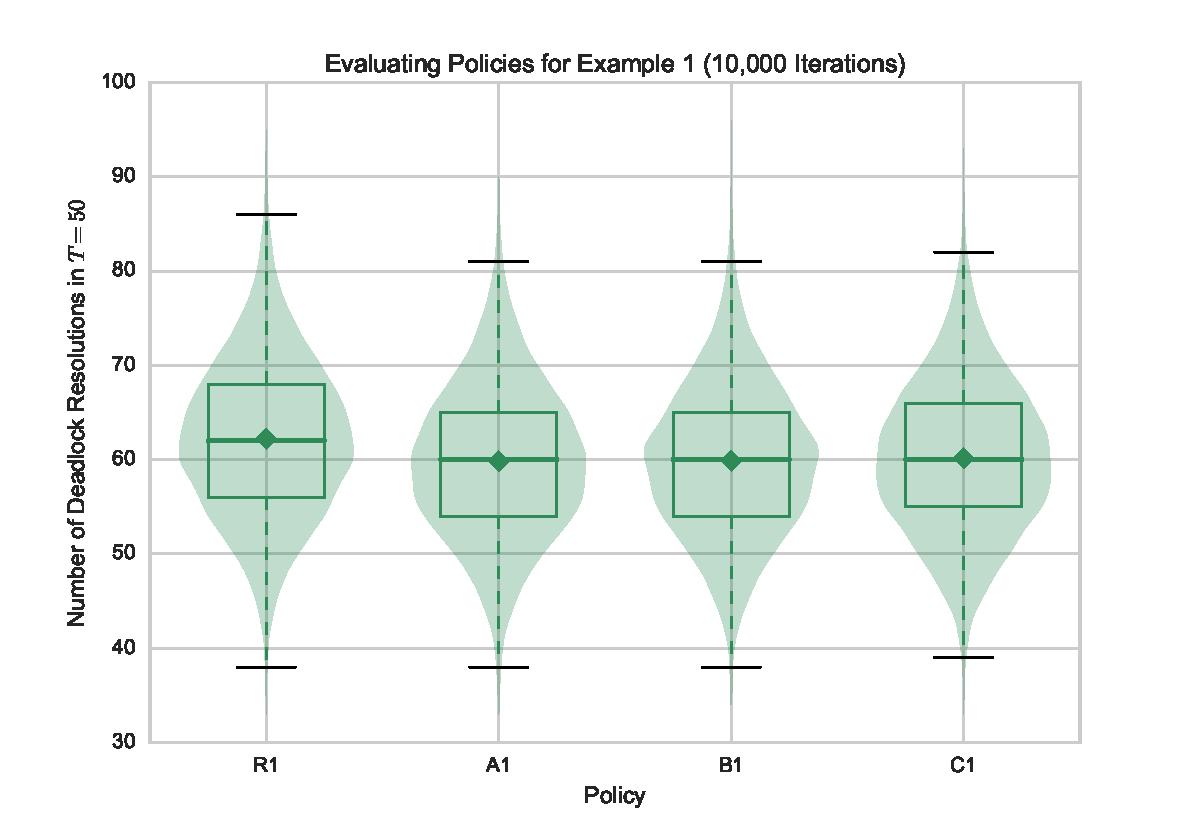
\includegraphics[width=0.98\textwidth]{../images/evaluation_example1.pdf}
\end{center}
\end{frame}

\end{document}
